\chapter{Analyse}
In diesem Kapitel wird die Problemlage im Bezug zum derzeitigen Stand der Technik analysiert.
Etablierte Verfahren, welche für eine Lösung geeignet wären, werden mithilfe von Bespielen aus der Literatur vorgestellt.
Anschließend werden die Verfahren mit einem geeigneten Testdatensatz evaluiert.
Hierbei werden auch die jeweilige Ressourcenlast und Effizienz gemessen.
Das geeignetste Verfahren wird für den weiteren Verlauf der Arbeit bestimmt.

\section{Stand der Technik}
Bildverarbeitung ist ein Thema, das schon sehr lange im Bereich der Informationstechnik und Informatik erforscht wird.
Besonders durch derzeitige Entwicklungen in der künstlichen Intelligenz und der Objekterkennung bekommt das Thema in der heutigen Zeit eine hohe Bedeutung für die technische Entwicklung. Im folgenden Kapitel werden einige der zum derzeitigen Zeitpunkt etablierten Verfahren der Bildverarbeitung im Kontext der Aufgabenstellung evaluiert und bewertet.

\subsection{Statische Verfahren}
Verfahren, welche ohne einen speziellen Kontext direkt auf die Pixelwerte eines Bildes angewendet werden können, werden im folgenden als "`statische Verfahren"' beschrieben. 

Diese Verfahren benötigen keine Vorverarbeitung oder Trainingsdaten, um verwendet zu werden.
In den meisten Fällen sind diese Verfahren besonders ressourceneffizient, da sie mit weniger Speicher- und Zeitkomplexität auskommen.
\subsubsection{Pixelorientierte Bildanalyse}
\textbf{Beschreibung}\newline
Ein trivialer Ansatz um Veränderungen zwischen zwei oder mehreren Bildern zu erkennen kann durch einen Vergleich der Pixelwerte ermöglicht werden.
So ist es auch möglich benachbarte Pixel in einem Bild nach bestimmten Veränderungen abzusuchen.
Bei den möglichen Veränderungen handelt es sich dabei um statistisch messbare Merkmale wie unter anderem auch Intensität, also Helligkeit, sowie die jeweiligen Farbwerte.

Helligkeits- oder Farbwechsel können im Bezug zur Objekterkennung auf einem Bild verwendet werden, indem man zum Beispiel eine Reihe an sogenannten "`Hintergrund"'-Pixeln wählt und diese mit den benachbarten Objektpixeln vergleicht.
Für den Fall der Verkehrskameras würde der besagte Hintergrund die Pixelwerte der Straße in dem gewählten Bereich beschreiben.
Sobald eine Reihe von Pixeln durch einen starken Farb- oder Intensitätswertwechsel unterbrochen wird, kann man in diesem Fall von einem beweglichen Objekt auf der Straße ausgehen.\newline\newline
\textbf{Literatur}\newline
O.K. Rahmat und Jumari beschreiben in ihrer Arbeit~\cite{bin2001vehicle} ein solches Verfahren und wenden dies auf Bilder von Verkehrskameras an. 
Die Besonderheit ist hierbei, dass nicht alle Pixelwerte des Bildes verglichen werden, sondern nur ein relevanter Teilabschnitt zu Vergleichszwecken ausgesucht wird. 
Dieser Teilbereich wird von den Autoren auch als "`Detektor"' beschrieben und befindet sich in der Mitte einer ausgewählten Fahrbahn. 
So werden auf Straßen mit mehreren Fahrbahnen auch mehrere solcher Detektoren benötigt.

Ziel ist es, wie bereits beschrieben die Intensität in dem Bereich eines Bildes zu überwachen. 
Sobald es einen stark abweichenden Wert gibt, wird davon ausgegangen, dass ein Auto den Streckenabschnitt des Detektors durchfährt und ein Zähler wird inkrementiert.
Die Länge eines stockenden Verkehrsflusses kann ebenfalls über diese Methode ermittelt werden. 
Hierfür wird in der Arbeit der beiden Autoren ein länglicher Detektor verwendet, der sich über den kompletten im Bild ersichtlichen Streckenabschnitt zieht.
Weiterhin werden die Farbwechsel innerhalb der Detektoren ausgewertet, um die einzelnen Objekte voneinander zu trennen.
\newline\newline
\textbf{Fazit}\newline
Das Verfahren hat eine sehr geringe Komplexität und ist daher einfach zu implementieren, jedoch werden auch schon in der Arbeit Situationen beschrieben in denen das Verfahren keine zuverlässigen Ergebnisse liefert. 
So kann zum Beispiel der Lichtkegel eines Scheinwerfers bei Nacht das Ergebnis verfälschen.
\begin{figure}[ht]
   \centering
     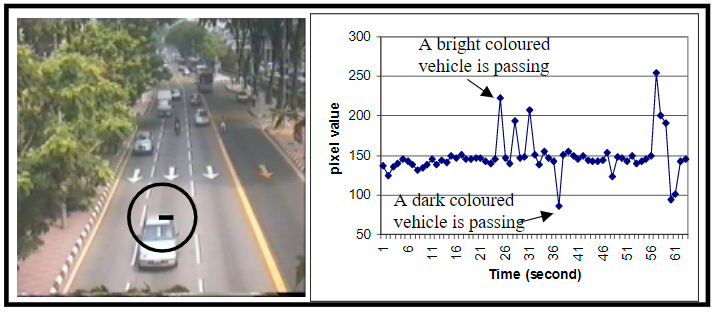
\includegraphics[width=15cm]{Bilder/pixelanalysis} \\
 \caption{Detektor im Einsatz}
 \sourceref{bin2001vehicle}
 \label{fig:Pixelanalysis}
\end{figure}
\newpage
\subsubsection{Kantenerkennung}
\textbf{Beschreibung}\newline
Kantenerkennung bezeichnet eine Klasse von Verfahren, bei welchen Kanten im Bild über abrupte Intensitätswert-Übergänge gefunden werden. 
Dabei werden in der Regel Faltungskerne (siehe \ref{sec:Faltungskerne}) verwendet, um die Ableitung der Intensitätswert-Funktion in einem Grauwert-Bild zu ermitteln.

Das bedeutet für die Anwendung des Verfahrens muss das Bild in den Grauwert-Bereich übertragen werden.
Die entstandenen Kanten (Abbildung~\ref{fig:gupte1}) können dann anschließend für die Objekterkennung verwendet werden. 
Um leicht überlagernde Objektkanten voneinander zu trennen können morphologische Operatoren verwendet werden (siehe \ref{sec:MorphologischeOperatoren}).
Diese werden auch verwendet, um kleine irrelevante Kanten aus dem Bild zu entfernen.
\newline\newline
\textbf{Literatur}\newline
Gupte und Papanikolopoulos stellen eine exemplarische Implementierung  des Verfahrens in ihrer Arbeit~\cite{gupte2000algorithms} vor. 
Dabei werden Kanten auf zwei Bildern einer Verkehrskamera erkannt und dann beide Kantenbilder per XOR vereinigt. 
Dies ermöglicht das Erkennen von Veränderungen zwischen den beiden Bildern der Verkehrskamera.
Mögliche Veränderungen können in diesem Fall auf ein bewegliches Objekt, wie zum Beispiel ein Auto, hindeuten.

Das Ergebnis wird anschließend mithilfe von der Anwendung von mehreren Dilatation-Operationen verbessert, da nicht geschlossene und im Objekt liegende Kanten zur einer großen Kante verbunden werden (Abbildung~\ref{fig:gupte2}).
Für den Fall das nach der Anwendung der jeweiligen Operationen immer noch unverbundene Kanten vorliegen werden nah benachbarte Kanten durch ein großes Rechteck umkreist.
Das resultierende Rechteck ist in diesem Fall dann das erkannte Objekt.
\newline\newline
\textbf{Fazit}\newline
Dieses Verfahren ist ebenfalls wenig komplex und lässt sich einfach implementieren. 
Jedoch besitzt es auch einige Nachteile, wie zum Beispiel, dass sich Schattenwurf negativ auf das Ergebnis auswirkt und eine Perspektive im Bild vorausgesetzt wird.
Wettereinflüsse wie Regen oder Schnee würden sich ebenfalls sehr negativ auf das Ergebnis auswirken.
Es existieren viele Implementierungen des Verfahrens, wobei die Arbeit von Gupte und Papanikolopoulos nur ein Beispiel ist.
So lassen sich auch durch Vorverarbeitung oder Maskierung der Bilder möglicherweise das Ergebnis verbessern.

\begin{figure}[ht]
  \centering
	\begin{minipage}[b]{0.4\textwidth}
     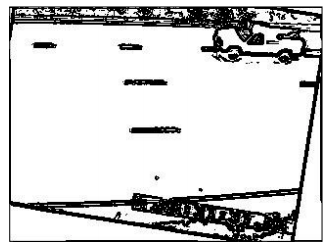
\includegraphics[width=\textwidth]{Bilder/gupte1} \\
   \caption{Kantenerkennung}
	 \sourceref{gupte2000algorithms}
   \label{fig:gupte1}
  \end{minipage}
	\hfill
	\begin{minipage}[b]{0.4\textwidth}
     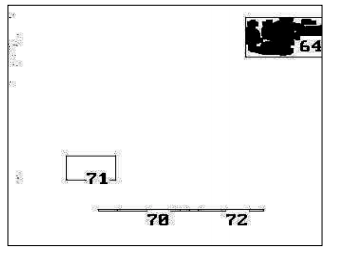
\includegraphics[width=\textwidth]{Bilder/gupte2} \\
		\caption{Ergebnis des~\newline Verfahrens}
	 \sourceref{gupte2000algorithms}
		\label{fig:gupte2}
	\end{minipage}
\end{figure}
\newpage

\subsection{Dynamische Verfahren}
Als "`dynamische Verfahren"' werden im folgenden Verfahren beschrieben, die nur innerhalb eines bestimmten Kontextes auf ein Bild angewendet werden sein. So kann es sein, dass das Verfahren bestimmte Trainingsdaten oder Vergleichswerte von anderen Bildern benötigt. Dies erhöht in den meisten Fällen die Genauigkeit des Verfahrens, aber die Ressourceneffizienz wird drastisch verringert.
\subsubsection{Neuronale Netze}
\textbf{Beschreibung}\newline
Neuronale Netze sind ein Beispiel für Verfahren aus dem maschinellen Lernen.
Hierbei wird versucht die Arbeitsweise des menschlichen Gehirns nachzuempfinden.
Neuronale Netze besitzen daher auch eine Art internen Speicher der antrainiertes Wissen abbildet.
Ein neuronales Netz kann somit für eine bestimmte Aufgabe trainiert werden, welche dann relativ zuverlässig von dem Netz gelöst werden kann.
Ziel von dem Training ist hierbei durch Anwendung des Netzes die Fehlerquote zu minimieren.
Sobald ein neuronales Netz fertig trainiert wurde, kann der Zustand des Netzes serialisiert und abgespeichert werden, damit es in der Zukunft weiterverwendet werden kann.
\newline\newline
\textbf{Literatur}\newline
In der Arbeit \cite{hkkDhbw} wurden sogenannte "`konvolutionale"' neuronale Netze für die Erkennung von stockendem Verkehr auf Bildern verwendet (siehe Abbildung~\ref{fig:CNN}).
Diese Netze nutzen unter anderem auch Faltungskerne (siehe~\ref{sec:Faltungskerne}) um Objektklassifizierung auf einem Bild durchzuführen.

Diverse Schichten von Neuronen werden in einem der verwendeten neuronalen Netze verwendet, um die aus den Pixelwerten gewonnenen Informationen auf eine konkrete Einschätzung bezüglich des Verkehrsflusses herunterzubrechen.
So kann eine Pixelmatrix als Eingabe an das neuronale Netzwerk weitergegeben werden und als Ausgabe ein einfacher boolescher Wert (eins oder null) empfangen werden. 
Eine Eins wäre beispielsweise eine positive Rückmeldung dafür, dass auf dem Bild stockender Verkehr sichtbar ist.

Wichtig hierbei sind die einzelnen Verbindungen zwischen den Neuronen-Schichten, welche je nach Training und Zustand des Netzes unterschiedlich gewichtet werden.
\begin{figure}[ht]
   \centering
     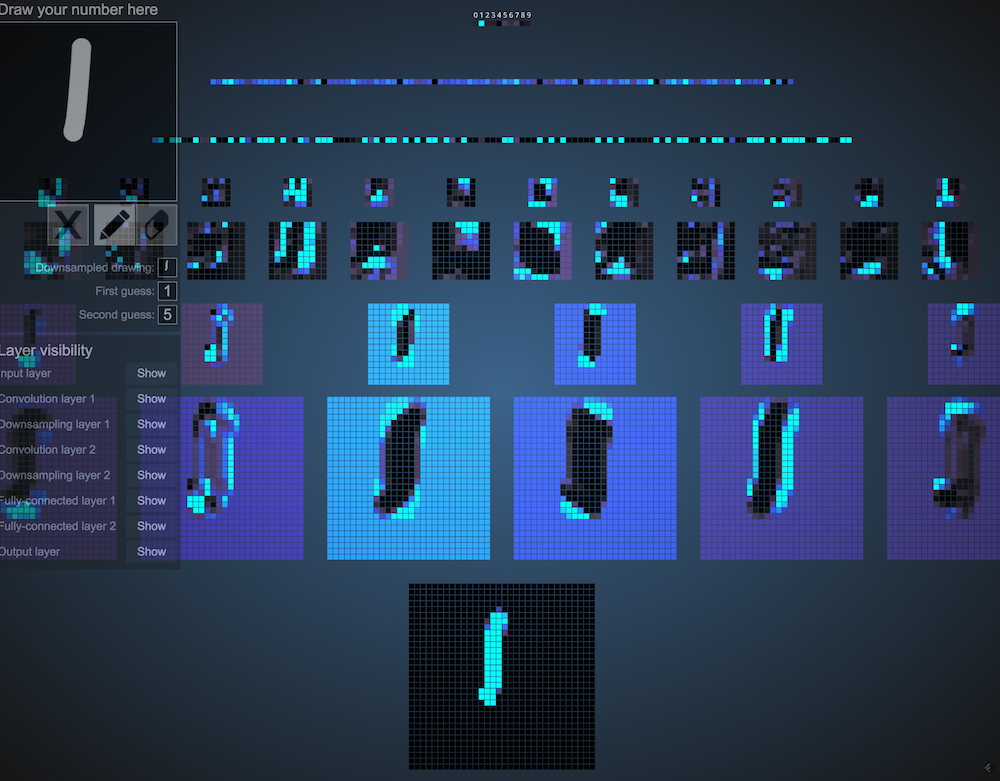
\includegraphics[width=15cm]{Bilder/cnn-visualized} \\
 \caption{Visualisierung der Schichten eines konvolutionalen neuronalen Netzwerks (unten Eingang - oben Ausgabe)}
 \source{http://scs.ryerson.ca/~aharley/vis/}{12.4.2019}
 \label{fig:CNN}
\end{figure}
\newline\newline
\textbf{Fazit}\newline
Bei der Laufzeit eines komplexen neuronalen fällt Netzes auf, dass das Laden und Benutzen der Neuronen einen relativ hohen Hauptspeicher-Bedarf mit sich bringt.
Der Vorteil der sich jedoch hierdurch bietet ist, dass Bilder nicht statisch analysiert werden, sondern das Netz dynamisch auf Bilder und Verhältnisse, wie zum Beispiel Perspektive und Wetter, trainiert wird.
Dieses Verfahren wurde für die folgende Implementierung nicht gewählt, da diese Arbeit einen besonderen Fokus auf die Ressourcensparsamkeit des Verfahrens setzt.
\newpage

\subsubsection{Background Subtraction}
\label{sec:backsub-algo}
\textbf{Beschreibung}\newline
Background Subtraction, auch als Foreground Detection bekannt, ist eine Klasse von Verfahren, bei denen einer Serie von Bildern auf Veränderungen analysiert wird.
Ziel ist es sich bewegende Objekte im Vordergrund des Bildes vom Hintergrund zu trennen.
Hierfür wird ein sogenanntes Hintergrund-Modell aus den ersten Bildern der Serie generiert, welches dann auf das letzte Bild angewendet wird, um ein Objekt im Vordergrund zu erkennen. 
Diese verwenden Statistiken, welche über alle Bilder der Serie generiert werden, um Gemeinsamkeiten zwischen den Bildern zu erkennen.

In dem Artikel \cite{mcivor2000background} werden mehrere dieser Hintergrund-Modelle im Detail beschrieben.
Bei der Auswahl des geeigneten Hintergrund-Modells sind mehrere Parameter zu berücksichtigen, wie zum Beispiel Perspektive und Farb- und Intensitäts-Spektrum.
\newline\newline
\textbf{Literatur}\newline
Akoum beschreibt im Artikel \cite{akoumBSIP} wie das Hintergrund-Modell "`Gaussian mixture Models"', oft auch als "`Mixtures of Gaussians"' beschrieben, auf ein Video einer Verkehrskamera angewandt werden kann.
Bei diesem Hintergrund-Modell werden alle Intensitätswerte der Pixel eines Bildes mithilfe eines Gaußschen Mischmodells modelliert.

Ein Gaußsches Mischmodell ist dabei ein statistisches Clusterverfahren, welches die Hintergrundpixel kategorisiert.
Alle Pixel, die nicht über das Mischmodell kategorisiert werden konnten sind somit Vordergrund-Pixel und somit auch mögliche Objekte im Vordergrund.
Objekte, die im Bild durch das Verfahren erkannt wurden sind im Anschluss weiß eingefärbt, während der Hintergrund schwarz eingefärbt wird.
Das Ergebnis des Verfahrens wird mit Dilatations- und Erosions-Filtern im Anschluss verbessert. 
Der Dilatations-Filter sorgt dabei für die Verbindung von nicht geschlossenen Kanten, während der Erosions-Filter kleine unwichtige Kanten aus dem Bild entfernt.
\newline\newline
\textbf{Fazit}\newline
Das Verfahren ist relativ komplex, bietet dafür aber eine sehr gute Genauigkeit. 
Aufgrund des Hintergrund-Modells müssen jedoch mehrere sich unterscheidende Bilder für das Verfahren verwendet werden.
Im Falle der Verkehrsanalyse sollte dies kein Problem darstellen, da eine fixierte Kamera bereits gegeben ist, welche jede Minute ein neues Bild aufnimmt.
Parameter die für das Anwenden des Hintergrund-Modells benötigt werden müssen im Hauptspeicher vorbehalten werden.
Daher hat dieses Verfahren auch nicht die beste Speichereffizienz.
Dennoch können durch die jeweiligen Hintergrund-Modelle auch Wetter- und Lichtveränderungen miteinbezogen werden, was potenzielle Fehlerquellen in den statischen Verfahren waren.
Weiterhin gibt es bereits einige Implementierungen diverser Hintergrund-Modelle in der Bibliothek OpenCV (siehe \ref{sec:OpenCV}).
\begin{figure}[!ht]
   \centering
     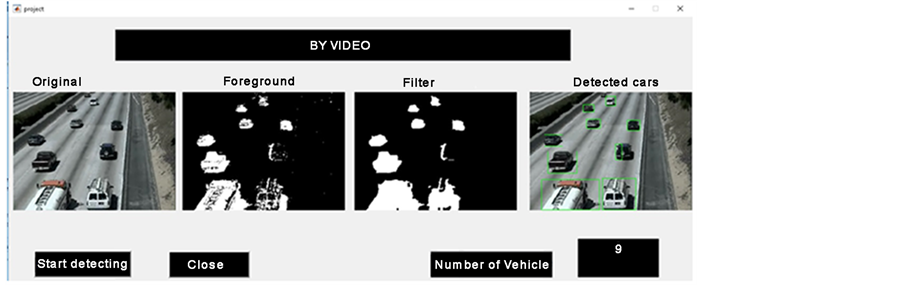
\includegraphics[width=15cm]{Bilder/mogpaper} \\
 \caption{Background Subtraction im Einsatz}
 \sourceref{akoumBSIP}
 \label{fig:BSSoftware}
\end{figure}
\newpage

\section{Bestimmung des Testdatensatzes}
\subsection{Verkehrskameras laden}
\label{sec:AnaCam}
Bevor die Kamerabilder geladen werden können, ist es zunächst relevant zu wissen welche Kameras es überhaupt gibt und wo diese liegen.
Hierfür stellt die Verkehrszentrale eine Liste aller Kameras unter dieser Webadresse bereit: \url{http://www.svz-bw.de/kamera/kamera_A.txt} (Stand: 31.3.2019).

Diese liegen in einer durch Tabulatorzeichen separierten Tabellenstruktur vor.

\begin{table}[ht]
  \centering
\scriptsize
    \begin{tabular}{ | l | l | l | l | l | l | l | l |}
    \hline
		lon & lat & title & description & linkextern & icon & iconSize & iconOffset \\ \hline
    572330.13 &
		5361095.33 &
		... &
		... &
		/.../kameradetail.php?id=EXT006 &
		... &
		16,16 &
		-8,-8 \\
    \hline
    \end{tabular}
		\caption{Tabellenstruktur der Kamerliste}
\end{table}

Die Werte {\em lat} und {\em lon} beschreiben die Position der Kamera durch Längen und Breitengrad.
Der Eintrag {\em title} enthält einen ausführlicheren Titel der Kamera. Mit {\em description} hat man die Möglichkeit eine detailliertere Beschreibung der Kamera zu erhalten, welche jedoch mit HTML Tags angereichert ist. {\em Linkextern} ist die Webadresse, über welche auf die Kamera zugegriffen werden kann. {\em Icon}, {\em iconSize} und {\em iconOffset} sind Informationen, die das Straßenverkehrszentrum selbst benötigt, um das Kameraicon auf einer Landkarte anzuzeigen.

Relevant sind also zunächst die Koordinaten, der Titel und der Link, da nur über diesen die ID der Kamera aufgelöst werden kann.
Das erste Problem hierbei ist, dass die Koordinaten der Kamera nicht der üblichen Projektion der Weltkugel entsprechen. Gebräuchlich ist die Projektion {\em WGS 84}~\cite{wgs84}, welche auch von Navigationssystemen oder herkömmlichen Kartendiensten genutzt wird und den Globus von -180° westlich bis 180° nördlich, bzw. -90° südlich bis 90° nördlich einteilt.

Das Straßenverkehrszentrum nutzt jedoch das Referenzsystem {\em ETRS89 / UTM zone 32N}~\cite{etrs89}, welches für Europa ausgelegt ist.
Um Position der Kameras mit gängigen Kartendiensten nutzen zu können, müssen die Koordinaten in die übliche Projektionsform überführt werden.

Außerdem muss die ID der Kamera aus dem Link extrahiert werden, da es keinen Eintrag in der Tabelle gibt, der lediglich die ID enthält.
Da der Link immer demselben Format folgt ({\em /<pfad>/kameradetail.php?id=<id>}), kann einfach nach dem Vorkommen der Teilzeichenkette {\em ?id=} gesucht werden, und alles davor abgeschnitten werden.

Somit lassen sich alle relevanten Informationen, welche für die Weiterverarbeitung der Kameras benötigt werden, abrufen.

\subsection{Verkehrsbilder laden}
Sobald die ID einer Kamera verfügbar ist, lassen sich auch die Kamerabilder abrufen.
Die Bilder werden im Regelfall alle 1-5 Minuten aktualisiert und im JPEG Format auf dem Server der Straßenverkehrszentrale öffentlich gemacht.
Es sind daher keine Videosequenzen, sondern nur Einzelbilder verfügbar.

Über die URL {\em https://www.svz-bw.de/kamera/ftpdata/<id>/<id>\_gross.jpg} lässt sich stets die aktuellste Aufnahme für eine Kamera abrufen, wobei {\em <id>} der ID der Kamera entsprechen muss.

Jedoch verbietet die Straßenverkehrszentrale den Zugriff auf die Bilder von außerhalb ihrer Webpräsenz.
Um dennoch darauf zugreifen zu können, kann der {\em Referer} HTTP-Header mit dem Hostnamen der Verkehrszentrale (http://svz-bw.de) beim Abrufen des Bildes mitgesendet werden, wodurch der Zugriff gewährt wird. 

\subsection{Vergleichsdatensätze generieren}
Bevor verschiedene Verfahren getestet und miteinander verglichen werden können, wird zunächst ein Vergleichsdatensatz benötigt.

Um nun den Datensatz zu generieren wird ein Python-Skript verwendet.
Wird dieses gestartet, fängt es an periodisch für einige der Kameras auf der A5 Bilder herunterzuladen.

Neben den Bildern selbst wird auch eine Metadatei im JSON-Format generiert.
Diese enthält zunächst einen Zeitstempel, wann das Bild erstellt wurde.
Außerdem enthält diese auch noch, wie viele Autos jeweils auf der linken und rechten Spur zu sehen sind, und ob anhand dessen Stau ist oder nicht.

Um diese Informationen zu generieren, wird ein sehr prototypischer Algorithmus verwendet. Die Resultate sind dementsprechend nicht gerade akkurat, weshalb ein Mensch diese zusätzlich verifizieren muss. Um jedoch den Menschen dabei zu unterstützen, ist eine grobe Vorauswertung sehr hilfreich.

Um als Mensch die Bilder auswerten zu können, kann ein zweites Skript Abhilfe schaffen.

Dazu gibt es in den Metadaten ein Feld, welches speichert, ob ein Bild bereits von einem Menschen verifiziert wurde.
Mit dem Skript werden nun nacheinander alle noch nicht ausgewerteten Bilder angezeigt, wobei abwechselnd die linke bzw. rechte Spur maskiert werden. Zusätzlich sieht man, ob die Vorauswertung für die angezeigte Spur Stau erkannt hat, oder nicht.

Als Mensch hat man nun die Möglichkeit durch das Drücken der Enter-Taste zu speichern, dass Stau auf dem Bild zu sehen ist, bzw. durch das Drücken einer anderen Taste zu bestätigen, dass kein Stau zu sehen ist.

Anschließend wird das nächste Bild bzw. die nächste Spur angezeigt.
Dies passiert solange, bis keine Bilder mehr ausgewertet werden müssen, bzw. der Nutzer das Skript beendet.

\section{Auswahl des Verfahrens}
Zur Auswahl des bestmöglichen Verfahrens werden verschiedene Ansätze anhand des Testdatensatzes ausgewertet.

\subsection{Helligkeit}
Das erste Verfahren klassifiziert ein Bild lediglich anhand der Häufigkeit der Intensitätswerte.
Dazu werden zunächst, wie beim Histogramm, die Intensitätswerte zwischen 0 und 255 aufsummiert.
Anhand eines Schwellwertes, in unserem Fall der Grauwert 40, wird dann versucht das Bild zu klassifizieren.
Gibt es in Summe mehr Grauwerte unter dem Schwellwert, als darüber, wird Stau auf dem Bild angenommen.
Die Überlegung dahinter ist, dass die Straße einen sehr neutralen bis hellen Grauton aufweist. Fahren nun Autos auf der Fahrbahn, dann können diese in verschiedensten Farben, sowohl über, als auch unter dem Schwellwert auftreten.
Jedoch werden von den Autos auch Schatten geworfen, welche die Straße verdunkeln, und so die Intensitätswerte reduzieren.
	
\subsection{Haar-Features}
Der Ansatz zur Stauerkennung über Haar-Features verläuft etwas anders als die Erkennung über die Helligkeit.
Hierbei wird versucht über Autos zu klassifizieren, um diese anschließend zu zählen und abzuschätzen, ob Stau ist, oder nicht.

Zur Klassifizierung der Autos kann ein von OpenCV mitgelieferter Cascade-Classifier zur Erkennung von Autos genutzt werden.
Dieser ist standardmäßig bei OpenCV verfügbar und soll über Haar-Features Autos auf Bildern erkennen können.
Solche Kaskaden werden als XML-Dateien mitgeliefert, welche über die Methode {\em CascadeClassifier} geladen werden können.

Anschließend kann damit ein Bild untersucht werden. Als Ergebnis erhält man eine Liste von Konturen, welche Autos auf dem Bild darstellen sollen.

Die Ergebnisse dieses Verfahrens sind jedoch nicht gut, falls die Auflösung der Kameras zu gering sind, da Merkmale von Autos nicht deutlich genug sind, um diese als Autos klassifizieren zu können.
Besser arbeiten Classifier auf Bild-Sequenzen, wie z.B. Videos, da diese dabei helfen Autos über die Sequenzen hinweg zu verfolgen.
Da die Straßenverkehrszentrale jedoch nur Einzelbilder liefert, sind die Ergebnisse nicht sehr genau.

\subsection{Edge-Detection}
Ein weiteres Verfahren, um Stau zu erkennen, kann mittels des Canny-Algorithmus umgesetzt werden.
Der Canny-Algorithmus erlaubt es Kanten innerhalb eines Bildes zu erkennen und verwendet dafür den Sobel-Operator~\ref{sec:Sobel}.

Umsetzen lässt sich der Algorithmus über die in OpenCV verfügbare Funktion {\em Canny}.
Dieser wandelt das Bild in ein Graustufenbild um, auf welchem die Kanten weiß dargestellt sind, und der Hintergrund schwarz.

Anschließend können über OpenCV die Konturen aus dem Bild entnommen werden und diese gezählt werden.
Die Zahl der Konturen sollte der Zahl der Autos entsprechen, wobei ein Teil davon den Hintergrund repräsentiert, welcher jedoch relativ statisch sein sollte, da sich der Hintergrund fast nie ändert.

Aufgrund der stark verrauschten Bilder der Kameras werden jedoch zu viele Kanten erkannt, um verlässlich Fahrzeuge erkennen zu können.
Eine vorherige Mittelung des Bildes mit Gauß verbessert das Ergebnis zwar, sorgt jedoch dafür, dass die Kanten nicht als getrennte Konturen ersichtlich werden, um von OpenCV entnommen werden zu können.
	
\subsection{Background-Subtraction}
Das Problem beim Canny-Algorithmus ist, dass der Hintergrund zu viel Einfluss auf das Resultat hatte.
Daher versucht dieser Ansatz den Hintergrund zu entfernen. Hierfür werden Background-Subtraction Techniken angewendet, die den Hintergrund
vom Hauptbild herausrechnen. Übrig bleiben sollten danach lediglich die Autos.

Der Background-Subtraction Algorithmus benötigt jedoch eine Reihe von Trainingsbildern, um zu lernen, was der Hintergrund ist.
Daher werden, bevor ein Bild analysiert werden kann, ca. 5-10 Vorlaufbilder benötigt.

Nun gibt es ebenfalls verschiedene Background-Subtraction Algorithmen, welche verwendet werden können. Beispielsweise gibt es {\em GSOC}, {\em KNN}, {\em MOG} oder {\em MOG2}, welche jeweils andere Ansätze verwenden, um den Hintergrund zu entfernen.

{\em MOG} liefert bei der Bildqualität der Kameras die besten Ergebnisse.

Der Algorithmus wird vor der Analyse also trainiert und berechnet anschließend ein Schwarz-Weiß-Bild, wobei weiße Pixel Objekte im Vordergrund darstellen.

Anhand der Konturenerkennung können dann Autos auf dem Bild gezählt werden. Bei überschreiten des Schwellwerts kann so Stau erkannt werden.

\subsection{Auswahl}
Für die Auswahl des Verfahrens werden die einzelnen Algorithmen und Verfahren anhand der Testdatensätze verglichen und bewertet.
Von insgesamt 252 Bildern gab es 62 auf denen Stau zu sehen ist und 190 ohne Stau.
Die Verfahren werden nun darauf getestet, wie gut sie Stau bei Bildern erkennen, die tatsächlich Stau andeuten (true positives), bzw. wie gut kein Stau auf Bildern ohne Stau erkannt wird (true negatives).

\paragraph{Vergleichsalgorithmus}
Dieser Algorithmus sagt für jedes Bild voraus, dass kein Stau zu sehen ist. Er dient zum Vergleich und soll sicherstellen, dass die Annahme "`kein Stau"' nicht besser sein kann, als mit den verwendeten Verfahren die Bilder tatsächlich auszuwerten.

\begin{table}[ht]
  \centering
\scriptsize
    \begin{tabular}{ | l | l | l |}
    \hline
		True Positives & True Negatives & Total \\ \hline
    0\% &
		100\% &
		76.86\% \\
    \hline
    \end{tabular}
		\caption{Ergebnisse des Vergleichsalgorithmus}
\end{table}

In 0\% der Fällen "`erkennt"' das Verfahren Stau der existiert, aber in 100\% der Fälle wird die Abwesenheit von Stau angenommen. Das bedeutet, dass die anderen Verfahren eine Gesamtgenauigkeit von 76.86\% bei diesem Testdatensatz übertreffen müssen, um einsatztauglich zu sein.

\paragraph{Helligkeitsvergleich}
In Bezug auf Ressourceneffizienz ist der Helligkeitsvergleich extrem gut, da sehr wenige primitive Berechnungen durchgeführt werden.
Jedoch liefert dieses Verfahren sehr schlechte Resultate. Unterschiedliche Tageszeiten, Lichtverhältnisse oder Autofarben haben einen zu großen Einfluss auf das Ergebnis, weshalb keine verlässlichen Ergebnisse generiert werden.

\begin{table}[ht]
  \centering
\scriptsize
    \begin{tabular}{ | l | l | l |}
    \hline
		True Positives & True Negatives & Total \\ \hline
    20\% &
		48\% &
		41.74\% \\
    \hline
    \end{tabular}
  \caption{Ergebnisse des Helligkeitsvergleichs}
\end{table}

In lediglich 20\% der Fälle, in denen Stau war, wurde auch tatsächlich Stau erkannt, bzw. nur in 48\% der Fälle in denen kein Stau war wurde auch kein Stau erkannt.
Mit einer Gesamtgenauigkeit von 41.74\% ist dieses Verfahren deutlich schlechter als der Vergleichsalgorithmus, weshalb es sich nicht für die weitere Entwicklung eignet.

\paragraph{Haar-Features}
Haar-Features liefen aufgrund der niedrigen Auflösung der Bilder keine verlässliche Erkennung von Autos. Bei einer höheren werden Autos zwar gut erkannt, aber nicht auf Bildern der Verkehrszentrale. Zusätzlich ist die Berechnung deutlich aufwendiger, was sich in Bezug auf Ressourcensparsamkeit negativ auswirkt.

\begin{table}[ht]
  \centering
\scriptsize
    \begin{tabular}{ | l | l | l |}
    \hline
		True Positives & True Negatives & Total \\ \hline
    0\% &
		100\% &
		76.86\% \\
    \hline
    \end{tabular}
  \caption{Ergebnisse der Haar-Features}
\end{table}

Zu erkennen ist, dass dieses Verfahren selben Ergebnisse wie der Vergleichsalgorithmus liefert. Es wird also gar nicht erst Stau erkannt, sondern bei jedem Bild davon ausgegangen es sei kein Stau. Daher eignet sich dieses Verfahren nicht.

\paragraph{Kantenerkennung}
Bei der Kantenerkennung ist die Ressourcensparsamkeit ziemlich gut erfüllt, da Kantenerkennung auf einfachen Faltungen basiert, welche sich effizient berechnen lassen.
Das Problem ist jedoch, dass Autos und Hintergrund nicht unterschieden werden können und Autos nicht verlässlich erkannt werden.

\begin{table}[ht]
  \centering
    \scriptsize
    \begin{tabular}{ | l | l | l |}
    \hline
		True Positives & True Negatives & Total \\ \hline
    30\% &
		77\% &
		67.36\% \\
    \hline
    \end{tabular}
  \caption{Ergebnisse der Kantenerkennung}
\end{table}

Mit einer Gesamtgenauigkeit von 67.36\% ist die Kantenerkennung zwar immer noch schlechter, als der Vergleichsalgorithmus, liefert jedoch immerhin in 30\% der Stau-Fälle eine korrekte Aussage, und sogar 77\% bei keinem Stau. Insgesamt sind die Ergebnisse jedoch viel zu ungenau, um für die weitere Arbeit zu genügen.

\paragraph{Background-Subtraction}
Background-Subtraction benötigt zwar Vorlaufbilder, welche zunächst von der Straßenverkehrszentrale nicht verfügbar sind, da lediglich das aktuellste Bild abgerufen werden kann, und nicht Bilder aus der Vergangenheit, jedoch ist nach Abschluss eines einmaligen Trainings der Algorithmus in der Lage jedes weitere Bild effizient zu verarbeiten. Zudem werden Autos verlässlich erkannt.

\begin{table}[ht]
  \centering
\scriptsize
    \begin{tabular}{ | l | l | l |}
    \hline
		True Positives & True Negatives & Total \\ \hline
    79\% &
		90\% &
		87.6\% \\
    \hline
    \end{tabular}
  \caption{Ergebnisse der Background-Subtraction}
\end{table}

Mit einer Gesamtgenauigkeit von 87.6\% ist Background-Subtraction das mit Abstand beste Verfahren. Im Gegensatz zum Vergleichsalgorithmus erkennt es zwar nur in 90\% der Fälle, dass kein Stau ist, wenn auch wirklich kein Stau ist, dafür erkennt es Stau in 79\% der Fälle und liefert ausreichend gute Ergebnisse für die Implementierung der Arbeit.
